
\documentclass[11pt,a4paper]{article}

\usepackage[T1]{fontenc}
\usepackage[utf8]{inputenc}
\usepackage[dutch]{babel}
\usepackage{lmodern}
\usepackage{microtype}
\usepackage[a4paper,margin=2.0cm]{geometry}
\usepackage{amsmath,amssymb}
\usepackage{booktabs,array,tabularx}
\usepackage{enumitem}
\usepackage{xcolor}
\usepackage{tikz}
\usetikzlibrary{arrows.meta,decorations.pathmorphing,positioning,calc,patterns,shapes.geometric}

\definecolor{notegray}{RGB}{245,245,245}
\definecolor{uncertain}{RGB}{145,70,0}
\definecolor{inkblue}{RGB}{28,78,150}
\definecolor{inkred}{RGB}{190,45,45}
\definecolor{inkgreen}{RGB}{35,135,75}
\definecolor{inkpurple}{RGB}{115,60,145}

\newcommand{\uncertain}[1]{\textcolor{uncertain}{\textit{[onzeker: #1]}}}
\newcommand{\literalnote}[1]{%
  \begin{center}
  \fcolorbox{black!35}{notegray}{%
    \begin{minipage}{0.92\linewidth}
      #1
    \end{minipage}}
  \end{center}
}
\newcommand{\photon}[3]{%
  \draw[#3,decorate,decoration={snake,amplitude=2pt,segment length=7pt},->,thick]
    (#1)--(#2);
}
\newcommand{\nucleus}[2]{%
  \fill[inkred!80] (#1,#2) circle (0.12);
}
\newcommand{\atomcloud}[4]{%
  \draw[#4,thick] (#1,#2) circle (#3);
  \draw[#4!75,thick] (#1,#2) circle ({0.72*#3});
  \nucleus{#1}{#2}
}

\title{\textbf{Kwantum Natuurkunde}\\
\large LaTeX-transcriptie van PDF-pagina's 11--15}
\author{}
\date{}

\begin{document}
\maketitle

\noindent
Deze transcriptie is gebaseerd op visuele inspectie van de oorspronkelijke
scans op hoge resolutie. De spelling en formulering zijn zoveel mogelijk
letterlijk behouden. Onduidelijke passages zijn gemarkeerd met
\uncertain{tekst}. De natuurkundige inhoud is niet stilzwijgend gecorrigeerd;
waar nuttig wordt een gangbare notatie afzonderlijk genoemd. De schetsen zijn
in TikZ gereconstrueerd.

% --------------------------------------------------------------------------
\section*{PDF-pagina 11 --- supergeleiderwetten}

\subsection*{Linker notitiepagina: ``Super geleider Wetten''}

De drie handgeschreven voorwaarden luiden:

\begin{enumerate}[label=\arabic*.,leftmargin=1.7em]
  \item Wanneer stof zo koud is dat de kern niet kan schuiven: B.E.C.
  \item Als de elektronen in harmonie gebracht worden door externe stimulatie.
  \item Wanneer de kernen in perfecte geometrische verhoudingen liggen:
        de afstand tussen elk naastliggend atoom is gelijk.
\end{enumerate}

Onder de tekst staan drie stadia van hetzelfde materiaal:

\begin{center}
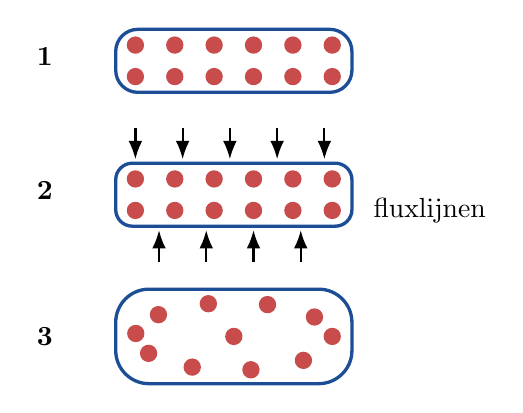
\begin{tikzpicture}[>=Latex,x=1cm,y=1cm]
  % stage 1
  \node[font=\bfseries] at (-5.8,1.8) {1};
  \draw[inkblue,very thick,rounded corners=8pt]
    (-4.9,1.35) rectangle (-1.9,2.15);
  \foreach \x in {-4.65,-4.15,-3.65,-3.15,-2.65,-2.15}
    \foreach \y in {1.55,1.95}
      \fill[inkred!85] (\x,\y) circle (0.11);

  % stage 2
  \node[font=\bfseries] at (-5.8,0.1) {2};
  \draw[inkblue,very thick,rounded corners=6pt]
    (-4.9,-0.35) rectangle (-1.9,0.45);
  \foreach \x in {-4.65,-4.15,-3.65,-3.15,-2.65,-2.15}
    \foreach \y in {-0.15,0.25}
      \fill[inkred!85] (\x,\y) circle (0.11);
  \foreach \x in {-4.65,-4.05,-3.45,-2.85,-2.25}
    \draw[->,thick] (\x,0.9)--(\x,0.5);
  \foreach \x in {-4.35,-3.75,-3.15,-2.55}
    \draw[->,thick] (\x,-0.8)--(\x,-0.4);
  \node[anchor=west] at (-1.75,-0.15) {fluxlijnen};

  % stage 3
  \node[font=\bfseries] at (-5.8,-1.75) {3};
  \draw[inkblue,very thick,rounded corners=12pt]
    (-4.9,-2.35) rectangle (-1.9,-1.15);
  \foreach \a in {0,35,...,325}
    \fill[inkred!85] ({-3.4+1.25*cos(\a)},{-1.75+0.43*sin(\a)}) circle (0.11);
  \fill[inkred!85] (-3.4,-1.75) circle (0.11);
\end{tikzpicture}
\end{center}

De tekst in het paarse kader is:

\literalnote{%
In een supergeleider zal door de harmonie elk elektron in harmonie komen en
functioneren als één. Hierdoor zal de kwantumexcitatie
\uncertain{op één plek tegelijk plaatsvinden / zijn}.}

\newpage
\subsection*{Rechter notitiepagina: nanobuis en spoel}

Bovenaan staat een perspectivische roosterconstructie met de labels
``Nanobuis'', ``Grafeen'' en ``een Super Geleider''.

\begin{center}
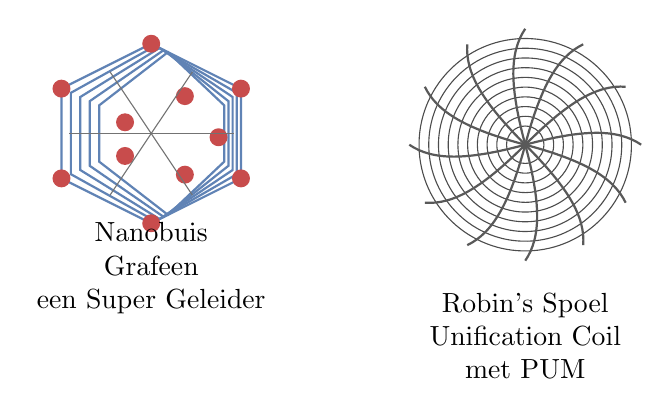
\begin{tikzpicture}[>=Latex,scale=0.95]
  % hexagonal nanotube tunnel
  \foreach \s in {0.0,0.28,0.56,0.84,1.12} {
    \draw[inkblue!70,thick]
      ({-3+0.45*\s},{1.55-0.20*\s}) --
      ({-1.8+0.20*\s},{2.15-0.10*\s}) --
      ({-0.6-0.20*\s},{1.55-0.20*\s}) --
      ({-0.6-0.20*\s},{0.35+0.20*\s}) --
      ({-1.8+0.20*\s},{-0.25+0.10*\s}) --
      ({-3+0.45*\s},{0.35+0.20*\s}) -- cycle;
  }
  \foreach \p in {(-3,1.55),(-1.8,2.15),(-0.6,1.55),(-0.6,0.35),(-1.8,-0.25),(-3,0.35),
                   (-2.15,1.1),(-1.35,1.45),(-0.9,0.9),(-1.35,0.4),(-2.15,0.65)}
    \fill[inkred!85] \p circle (0.12);
  \foreach \a in {0,60,...,300}
    \draw[black!55] (-1.8,0.95)--({-1.8+1.1*cos(\a)},{0.95+0.95*sin(\a)});
  \node[align=center] at (-1.8,-0.85)
    {Nanobuis\\Grafeen\\een Super Geleider};

  % spiral/coil
  \begin{scope}[shift={(3.2,0.8)}]
    \foreach \r in {0.25,0.38,...,1.55}
      \draw[black!70,rotate=\r] (0,0) circle (\r);
    \foreach \a in {0,30,...,330}
      \draw[black!65,thick] (0,0) .. controls
        ({0.8*cos(\a+15)},{0.8*sin(\a+15)}) and
        ({1.25*cos(\a+10)},{1.25*sin(\a+10)}) ..
        ({1.55*cos(\a)},{1.55*sin(\a)});
    \node[align=center,below] at (0,-1.85)
      {Robin's Spoel\\Unification Coil\\met PUM};
  \end{scope}
\end{tikzpicture}
\end{center}

% --------------------------------------------------------------------------
\section*{PDF-pagina 12 --- energieniveaus en dodeca-symmetrie}

\subsection*{Linker notitiepagina: energieniveaus}

De scan toont de gebruikelijke waterstofniveaus:

\begin{center}
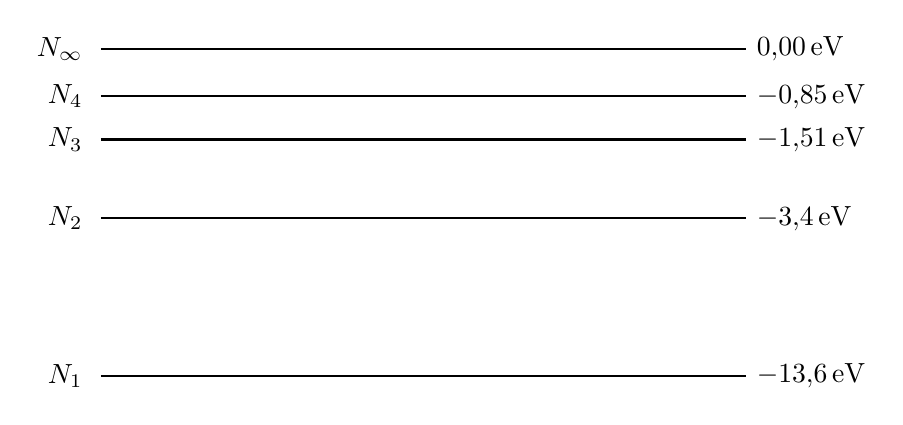
\begin{tikzpicture}[x=1cm,y=1cm]
  \draw[thick] (0,0.2)--(8.2,0.2)
    node[left=8.3cm] {$N_1$} node[right] {$-13{,}6\,\mathrm{eV}$};
  \draw[thick] (0,2.2)--(8.2,2.2)
    node[left=8.3cm] {$N_2$} node[right] {$-3{,}4\,\mathrm{eV}$};
  \draw[thick] (0,3.2)--(8.2,3.2)
    node[left=8.3cm] {$N_3$} node[right] {$-1{,}51\,\mathrm{eV}$};
  \draw[thick] (0,3.75)--(8.2,3.75)
    node[left=8.3cm] {$N_4$} node[right] {$-0{,}85\,\mathrm{eV}$};
  \draw[thick] (0,4.35)--(8.2,4.35)
    node[left=8.3cm] {$N_{\infty}$} node[right] {$0{,}00\,\mathrm{eV}$};
\end{tikzpicture}
\end{center}

\literalnote{%
Elektron in baan $N_2$ doet excitatie naar level $N_3$ door een foton uit te
stralen met de frequentie.}

De vergelijking is geschreven als:

\begin{align*}
f &= \frac{E}{h}
   = \frac{E_2-E_1}{h}
   = \frac{c}{\lambda}.
\end{align*}

Bij een overgang tussen twee niveaus kan de fotonfrequentie genormaliseerd
worden geschreven als
\[
f=\frac{\lvert E_{\mathrm{hoog}}-E_{\mathrm{laag}}\rvert}{h}.
\]

\newpage
\subsection*{Rechter notitiepagina: geometrische symmetrie}

Bovenaan staan drie schetsregels:

\begin{align*}
5\times \triangle &\;=\; \text{Dodeca},\\
5\times \text{vijfhoek} &\;=\; \text{Dodeca},\\
5\times \uncertain{\text{veelvlak}} &\;=\; \text{Dodeca}.
\end{align*}

Daaronder staat:
\[
\text{Tetra--octa cube}\quad 32^\circ,
\qquad
\text{dodeca--icosa symmetry}.
\]

Links van de samengestelde stervorm staat $0{,}618$. De groene notitie toont
schematisch een samentelling van een opwaartse en een neerwaartse tetraëder:

\begin{center}
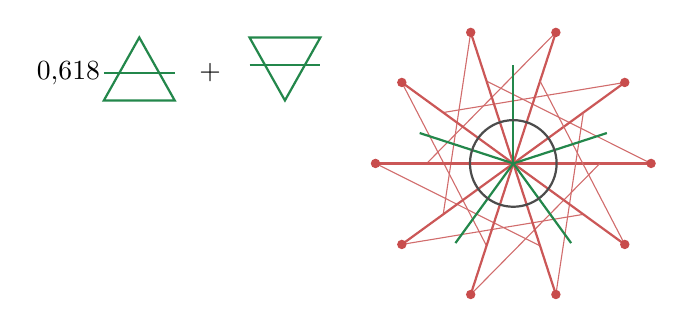
\begin{tikzpicture}[scale=1.0]
  % two small tetrahedra
  \draw[inkgreen,thick] (-4,1.2)--(-3.55,2.0)--(-3.1,1.2)--cycle;
  \draw[inkgreen,thick] (-4,1.55)--(-3.1,1.55);
  \node at (-2.65,1.55) {$+$};
  \draw[inkgreen,thick] (-2.15,2.0)--(-1.7,1.2)--(-1.25,2.0)--cycle;
  \draw[inkgreen,thick] (-2.15,1.65)--(-1.25,1.65);
  \node at (-4.45,1.55) {$0{,}618$};

  % compound star
  \begin{scope}[shift={(1.2,0.4)}]
    \foreach \a in {0,36,...,324} {
      \draw[inkred!80,thick] (0,0)--({1.75*cos(\a)},{1.75*sin(\a)});
      \draw[inkred!70] ({1.75*cos(\a)},{1.75*sin(\a)})--
        ({1.1*cos(\a+108)},{1.1*sin(\a+108)});
      \fill[inkred!85] ({1.75*cos(\a)},{1.75*sin(\a)}) circle (0.06);
    }
    \foreach \a in {18,90,...,306}
      \draw[inkgreen,thick] (0,0)--({1.25*cos(\a)},{1.25*sin(\a)});
    \draw[black!70,thick] (0,0) circle (0.55);
  \end{scope}
\end{tikzpicture}
\end{center}

% --------------------------------------------------------------------------
\newpage
\section*{PDF-pagina 13 --- vrije val, absorptie en Dopplereffect}

\subsection*{Linker notitiepagina: vallen in vacuüm}

De kop luidt: ``alles op aarde valt even snel in een vacuüm''.

\begin{center}
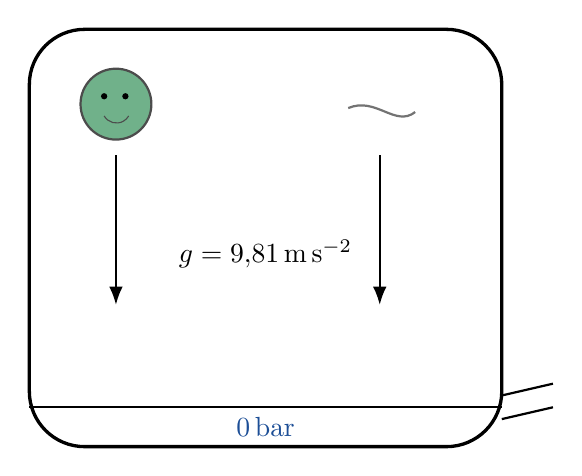
\begin{tikzpicture}[>=Latex,x=1cm,y=1cm]
  \draw[very thick,rounded corners=20pt] (-3,-2.5) rectangle (3,2.8);
  \draw[thick] (-3,-2.0)--(3,-2.0);
  \node[inkblue,font=\bfseries] at (0,-2.25) {$0\,\mathrm{bar}$};
  \fill[inkgreen!65] (-1.9,1.85) circle (0.45);
  \draw[black!70,thick] (-1.9,1.85) circle (0.45);
  \fill[black] (-2.05,1.95) circle (0.04);
  \fill[black] (-1.78,1.95) circle (0.04);
  \draw[black!70] (-2.05,1.70) arc (210:330:0.18);
  \draw[black!55,thick] (1.05,1.8).. controls (1.4,1.95) and
    (1.65,1.55)..(1.9,1.75);
  \draw[->,thick] (-1.9,1.2)--(-1.9,-0.7);
  \draw[->,thick] (1.45,1.2)--(1.45,-0.7);
  \node at (0,-0.05) {$g=9{,}81\,\mathrm{m\,s^{-2}}$};
  \draw[thick] (3,-2.15)--(3.65,-2.0);
  \draw[thick] (3,-1.85)--(3.65,-1.7);
\end{tikzpicture}
\end{center}

\literalnote{%
Dus massa heeft geen invloed op de zwaartekracht in een vacuüm. Hetzelfde
geldt dus ook in de ruimte \ldots}

Onderaan staat in groter schrift:

\literalnote{%
Alles valt even snel, dus Dopler effect heeft geen invloed.}

\subsection*{Rechter notitiepagina: twee lichamen die elkaar naderen}

De genummerde tekening toont twee identieke lichamen die aanvankelijk licht
uitstralen, het licht van elkaar absorberen, versnellen en uiteindelijk naast
elkaar komen.

\begin{center}
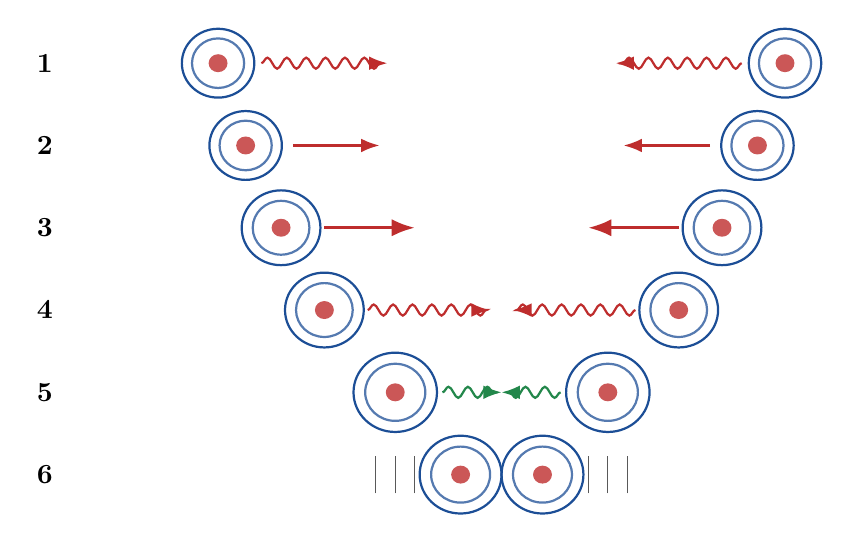
\begin{tikzpicture}[>=Latex,x=1cm,y=0.95cm]
  \foreach \y/\n in {4.2/1,3.1/2,2.0/3,0.9/4,-0.2/5,-1.3/6}
    \node[font=\bfseries] at (-5.8,\y) {\n};

  % row 1
  \atomcloud{-3.6}{4.2}{0.46}{inkblue}
  \atomcloud{3.6}{4.2}{0.46}{inkblue}
  \photon{-3.05,4.2}{-1.45,4.2}{inkred}
  \photon{3.05,4.2}{1.45,4.2}{inkred}

  % row 2
  \atomcloud{-3.25}{3.1}{0.46}{inkblue}
  \atomcloud{3.25}{3.1}{0.46}{inkblue}
  \draw[->,thick,inkred] (-2.65,3.1)--(-1.55,3.1);
  \draw[->,thick,inkred] (2.65,3.1)--(1.55,3.1);

  % row 3
  \atomcloud{-2.8}{2.0}{0.50}{inkblue}
  \atomcloud{2.8}{2.0}{0.50}{inkblue}
  \draw[->,very thick,inkred] (-2.25,2.0)--(-1.1,2.0);
  \draw[->,very thick,inkred] (2.25,2.0)--(1.1,2.0);

  % row 4
  \atomcloud{-2.25}{0.9}{0.50}{inkblue}
  \atomcloud{2.25}{0.9}{0.50}{inkblue}
  \photon{-1.7,0.9}{-0.15,0.9}{inkred}
  \photon{1.7,0.9}{0.15,0.9}{inkred}

  % row 5
  \atomcloud{-1.35}{-0.2}{0.53}{inkblue}
  \atomcloud{1.35}{-0.2}{0.53}{inkblue}
  \photon{-0.75,-0.2}{0,-0.2}{inkgreen}
  \photon{0.75,-0.2}{0,-0.2}{inkgreen}

  % row 6
  \atomcloud{-0.52}{-1.3}{0.52}{inkblue}
  \atomcloud{0.52}{-1.3}{0.52}{inkblue}
  \foreach \x in {-1.6,-1.35,-1.1,1.1,1.35,1.6}
    \draw[black!65] (\x,-1.55)--(\x,-1.05);
\end{tikzpicture}
\end{center}

De blauwe en rode aantekeningen luiden:

\literalnote{%
Twee lichamen met $v=0\,\mathrm{m/s}$ stralen licht uit \ldots{} Door de
absorptie komt het lichaam in beweging \ldots{} Het Dopler effect zorgt voor
een hogere frequentie, dus meer energie.}

De formules onderaan zijn:
\begin{align*}
E_k &= h f,\\
E_k &= \frac{1}{2}mv^2.
\end{align*}

% --------------------------------------------------------------------------
\newpage
\section*{PDF-pagina 14 --- foton--elektron en frequentie}

\subsection*{Linker notitiepagina: ``foton--Elektron''}

De bovenste reeks toont een botsing waarna het getekende object steeds kleiner
wordt en uiteindelijk in twee kleine componenten eindigt.

\begin{center}
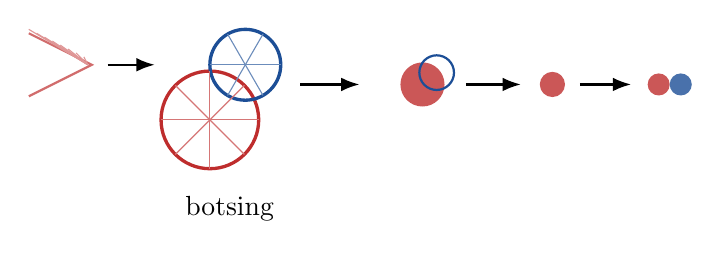
\begin{tikzpicture}[>=Latex,x=1cm,y=1cm]
  \draw[inkred!70,thick] (-5,1.2)--(-4.2,0.8)--(-5,0.4);
  \foreach \i in {0,...,7}
    \draw[inkred!50] (-5+0.1*\i,1.25-0.05*\i)--(-4.25,0.8);
  \draw[->,thick] (-4.0,0.8)--(-3.4,0.8);

  \draw[inkred,very thick] (-2.7,0.1) circle (0.62);
  \draw[inkblue,very thick] (-2.25,0.8) circle (0.45);
  \foreach \a in {0,45,...,315}
    \draw[inkred!65] (-2.7,0.1)--({-2.7+0.62*cos(\a)},{0.1+0.62*sin(\a)});
  \foreach \a in {0,60,...,300}
    \draw[inkblue!65] (-2.25,0.8)--({-2.25+0.45*cos(\a)},{0.8+0.45*sin(\a)});
  \node[below] at (-2.45,-0.75) {botsing};
  \draw[->,thick] (-1.55,0.55)--(-0.8,0.55);

  \fill[inkred!80] (0,0.55) circle (0.28);
  \draw[inkblue,thick] (0.18,0.7) circle (0.22);
  \draw[->,thick] (0.55,0.55)--(1.25,0.55);
  \fill[inkred!80] (1.65,0.55) circle (0.16);
  \draw[->,thick] (2.0,0.55)--(2.65,0.55);
  \fill[inkred!80] (3.0,0.55) circle (0.14);
  \fill[inkblue!80] (3.28,0.55) circle (0.14);
\end{tikzpicture}
\end{center}

Daaronder worden rood en paars licht naast elkaar gezet:

\begin{center}
\begin{tabularx}{\linewidth}{>{\centering\arraybackslash}X|
                              >{\centering\arraybackslash}X}
\textbf{Rood licht} & \textbf{Paars licht}\\[2mm]
lange $\lambda$ & korte $\lambda$\\
grote elektron & kleine elektron\\
onduidelijke locatie of snelheid &
duidelijke locatie of snelheid
\end{tabularx}
\end{center}

\begin{center}
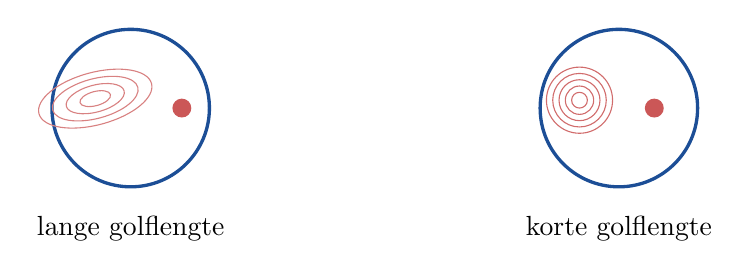
\begin{tikzpicture}[x=1cm,y=1cm]
  % red / broad distribution
  \draw[inkblue,very thick] (-3.1,0) circle (1.0);
  \foreach \r in {0.2,0.38,...,0.9}
    \draw[inkred!60,rotate around={15:(-3.55,0.12)}] (-3.55,0.12) ellipse [x radius=\r,y radius={0.45*\r}];
  \nucleus{-2.45}{0}
  \node[below] at (-3.1,-1.25) {lange golflengte};

  % violet / localized
  \draw[inkblue,very thick] (3.1,0) circle (1.0);
  \foreach \r in {0.10,0.18,...,0.42}
    \draw[inkred!70] (2.6,0.1) circle (\r);
  \nucleus{3.55}{0}
  \node[below] at (3.1,-1.25) {korte golflengte};
\end{tikzpicture}
\end{center}

Onderaan staan twee zeer lichte, moeilijk leesbare breuken. Ze lijken beide
de vorm te hebben
\[
c=\frac{\textcolor{uncertain}{\varepsilon\ \text{of}\ E}\,\lambda^2}
        {0{,}5\,\lambda},
\]
met daarnaast respectievelijk de labels ``grote foton'' en ``kleine foton''.
De tweede teller bevat mogelijk een subscript $0$.

\subsection*{Rechter notitiepagina: energie en kracht}

De tekst en vergelijkingen zijn:

\begin{align*}
E &= h f,\\
E &= \frac{\lVert\mathbf{F}\rVert}{Q}.
\end{align*}

\literalnote{%
Dopler geeft hogere $f$. Wanneer $f$ hoger wordt, wordt $E$ hoger.
$Q$ is vast en verandert niet. Dus als $E$ hoger wordt, wordt
$\mathbf{F}$ ook hoger. Hierdoor trekt de kern opzij.}

% --------------------------------------------------------------------------
\newpage
\section*{PDF-pagina 15 --- elektronengolf en lokalisatie}

\subsection*{Linker notitiepagina: statische elektronengolf}

Bovenaan staat:

\literalnote{%
Een atoom heeft in een normale staat een elektronengolf.}

De eerste schets wordt ``een uitsnede'' genoemd. De tweede is beschreven als
``een realistischer 3D-look van een statisch atoom''.

\begin{center}

\begin{tikzpicture}[x=1cm,y=1cm]
  % cross section
  \draw[inkblue,very thick,rounded corners=10pt]
    (-4.5,1.1) .. controls (-4.0,1.75) and (-3.35,1.25) ..
    (-3.2,0.55) .. controls (-3.0,-0.1) and (-4.1,-0.35) ..
    (-4.55,0.15) .. controls (-4.9,0.55) and (-4.85,0.85) .. cycle;
  \nucleus{-4.0}{0.6}
  \node[right] at (-3.0,0.65) {een uitsnede};

  % 3-D cloud
  \begin{scope}[shift={(1.8,0.45)}]
    \foreach \a in {0,18,...,162}
      \draw[inkblue!55,rotate=\a] (0,0) ellipse (1.4 and 0.58);
    \foreach \a in {0,30,...,150}
      \draw[inkred!55,rotate=\a] (0,0) ellipse (0.75 and 0.32);
    \nucleus{0}{0}
  \end{scope}
  \node[align=left] at (4.5,0.4)
    {een realistischer\\3D-look van een\\statisch atoom};
\end{tikzpicture}
\end{center}

Daaronder staat:

\literalnote{%
Wanneer een foton tegen de elektronengolf botst, klapt de golf in.}

\begin{center}
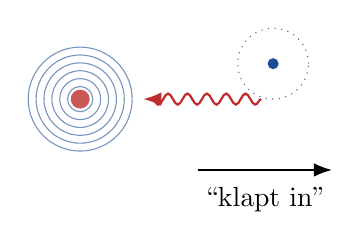
\begin{tikzpicture}[>=Latex,x=1cm,y=1cm]
  \foreach \r in {0.16,0.26,...,0.66}
    \draw[inkblue!60] (-2.5,0) circle (\r);
  \nucleus{-2.5}{0}
  \photon{-0.2,0}{-1.7,0}{inkred}
  \fill[inkblue] (-0.05,0.45) circle (0.07);
  \draw[dotted,black!60] (-0.05,0.45) circle (0.45);
  \draw[->,thick] (-1.0,-0.9)--(0.7,-0.9);
  \node[below] at (-0.15,-1.0) {``klapt in''};
\end{tikzpicture}
\end{center}

\subsection*{Rechter notitiepagina: golf en deeltje}

De eerste alinea luidt:

\literalnote{%
Een elektronengolf reageert als een complete golf en is dus in balans om de
proton.}

Daaronder:

\literalnote{%
Wanneer de elektron als deeltje zichtbaar is bij een interferentie met een
foton, reageert het als een deeltje.}

De drie vakken zijn schematisch:

\begin{center}
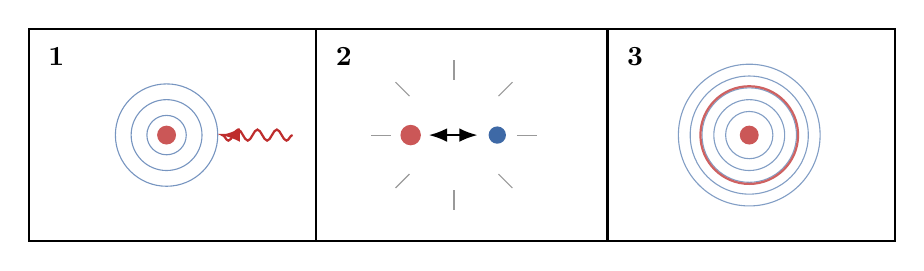
\begin{tikzpicture}[>=Latex,x=1cm,y=1cm]
  \draw[thick] (-5.5,-1.35) rectangle (5.5,1.35);
  \draw[thick] (-1.85,-1.35)--(-1.85,1.35);
  \draw[thick] (1.85,-1.35)--(1.85,1.35);
  \node[font=\bfseries] at (-5.15,1.0) {1};
  \node[font=\bfseries] at (-1.5,1.0) {2};
  \node[font=\bfseries] at (2.2,1.0) {3};

  \foreach \r in {0.25,0.45,0.65}
    \draw[inkblue!60] (-3.75,0) circle (\r);
  \nucleus{-3.75}{0}
  \photon{-2.15,0}{-3.05,0}{inkred}

  \fill[inkred!80] (-0.65,0) circle (0.13);
  \fill[inkblue!85] (0.45,0) circle (0.11);
  \draw[<->,thick] (-0.42,0)--(0.20,0);
  \foreach \a in {0,45,...,315}
    \draw[black!40] ({-0.1+0.8*cos(\a)},{0.7*sin(\a)})--({-0.1+1.05*cos(\a)},{0.95*sin(\a)});

  \foreach \r in {0.3,0.45,...,0.9}
    \draw[inkblue!55] (3.65,0) circle (\r);
  \draw[inkred!75,thick] (3.65,0) circle (0.62);
  \nucleus{3.65}{0}
\end{tikzpicture}
\end{center}

De afsluitende tekst is gedeeltelijk vaag:

\literalnote{%
Wanneer je een grotere $\lambda$ hebt in de foton, is het moeilijker te
bepalen waar de elektron is, omdat de golf een groter
\uncertain{deeltje/gebied} bestrijkt. Hoe meer energie/frequentie het foton
heeft, hoe preciezer de elektron \uncertain{bepaald kan zijn}.}

\end{document}
